\documentclass[tikz]{standalone}
\usepackage{amsmath,amssymb}
\usepackage{pgfplots,multicol}

\pgfplotsset{compat=1.10}
\usepgfplotslibrary{fillbetween}

\begin{document}


 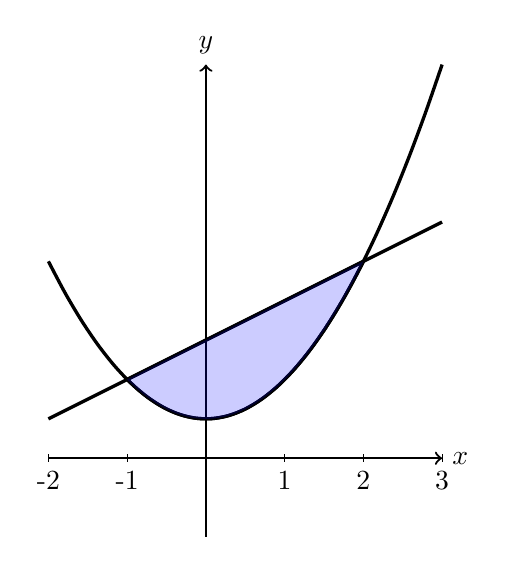
\begin{tikzpicture}[xscale=1,yscale=0.5]
        \draw[->,thick] (-2,0) -- (3,0) node[right] {$x$};
    \draw[->,thick] (0,-2) -- (0,10) node[above] {$y$};
	\foreach \x in {-2,-1,1,2,3} \draw (\x,0.1) -- (\x, -0.1) node[below] {\x};
	%\foreach \y in {-5,5} \draw (0.1,\y) -- (-0.1, \y) node[left] {\y};
	\draw[-,name path=A,smooth,domain=-1:2,very thick,black] plot(\x,{\x*\x+1});
	\draw[-,name path=B,smooth,domain=-1:2,very thick,black] plot(\x,{\x+3});
	\draw[-,smooth,domain=-2:3,very thick,black] plot(\x,{\x*\x+1});
	\draw[-,smooth,domain=-2:3,very thick,black] plot(\x,{\x+3});
	\tikzfillbetween[of=A and B]{blue, opacity=0.2};
	%\draw [fill=white] (2,0.1) circle[radius= 0.3 em]; 
	%\draw[] (3,5) node[right] {$-x^2+4x+3$};
	%\draw[] (3,8) node[right] {$-x^3+7x^2-10x+5$};
\end{tikzpicture}



	
\end{document}
